\documentclass[12pt]{article}
\usepackage[top=1.8cm,bottom=1.8cm,left=2cm,right=2cm]{geometry}
\usepackage[dvipsnames,svgnames,x11names]{xcolor}
\usepackage{graphicx}
\usepackage{array}
\usepackage{booktabs}
\usepackage{multicol}
\usepackage{enumitem}
\usepackage{tikz}
\usetikzlibrary{shapes.geometric, arrows.meta, positioning, fit, backgrounds, calc}
\setlength{\parindent}{0pt}
\setlength{\parskip}{4pt}
\usepackage[hidelinks]{hyperref}
\usepackage{caption}
\captionsetup{font=small, labelfont=bf, skip=4pt}

% ── Colour palette ──────────────────────────────────────────────
\definecolor{clientbg}{RGB}{219,234,254}
\definecolor{backbg}{RGB}{220,252,231}
\definecolor{dbbg}{RGB}{254,243,199}
\definecolor{modbg}{RGB}{237,233,254}
\definecolor{boxborder}{RGB}{100,116,139}
\definecolor{layerA}{RGB}{191,219,254}
\definecolor{layerB}{RGB}{187,247,208}
\definecolor{layerC}{RGB}{253,230,138}

\tikzset{
  sysbox/.style={rectangle, rounded corners=3pt, draw=boxborder,
                 fill=#1, minimum width=2.2cm, minimum height=0.65cm,
                 font=\footnotesize\bfseries, align=center, inner sep=4pt},
  modbox/.style={rectangle, rounded corners=3pt, draw=boxborder,
                 fill=modbg, minimum width=1.9cm, minimum height=0.6cm,
                 font=\scriptsize, align=center},
  dbbox/.style={rectangle, rounded corners=3pt, draw=boxborder,
                fill=dbbg, minimum width=1.8cm, minimum height=0.6cm,
                font=\scriptsize, align=center},
  arrowstyle/.style={-{Stealth[length=4pt]}, thick, color=boxborder},
  layerbox/.style={rectangle, rounded corners=4pt, draw=boxborder,
                   fill=#1, minimum width=6cm, minimum height=0.8cm,
                   font=\small\bfseries, align=center},
}

\begin{document}

% ── Header & Metadata ──────────────────────────────────────────
\begin{center}
\includegraphics[scale=0.44]{header.png}
\end{center}
\begin{flushright}
Date: March 11, 2025
\end{flushright}
\begin{center}
\textbf{\large Review I} \\ Project Phase -- II (CSL702/ITL702)
\end{center}
\vspace{0.15cm}
\begin{tabular}{|p{4cm}|p{4cm}|p{4cm}|p{4cm}|}
\hline
--&  \textbf{Student No. 1} & \textbf{Student No. 2} & \textbf{Student No. 3} \\  \hline
\textbf{Student Name} & Kshitiz Raj & Sujal Agrawal & Krishna Goswami\\ \hline
\textbf{Roll No.} & 23333 & 23358 & 23331\\ \hline
\textbf{Batch No.}& B-22 & \textbf{Semester} & 6th\\
\hline
 \textbf{Branch}& IT & \textbf{Supervisor(s)} & Mrs. Akansha Moral\\
\hline
\end{tabular}
\vspace{0.25cm}
\begin{center}
\textbf{\LARGE ResQNet --- Community Volunteer Emergency Response Network}
\end{center}

% ── 1. Introduction ─────────────────────────────────────────────
\section{Introduction}
ResQNet is a location-aware mobile and web platform that connects individuals experiencing emergencies with nearby community volunteers in real time. When a user triggers an SOS, the system identifies, ranks, and notifies the closest available volunteers using geospatial indexing; the first volunteer who accepts is matched to the requester, and a live coordination channel is established. The platform comprises an \textbf{Android application} (Kotlin, Jetpack Compose) serving both requester and volunteer roles, an \textbf{admin web dashboard} (Next.js) for platform oversight, and a \textbf{modular monolith backend} (Node.js/TypeScript) backed by PostgreSQL with PostGIS for spatial queries, Redis for real-time pub/sub and caching, and Firebase Cloud Messaging for push notifications. The high-level architecture is illustrated in Figure~\ref{fig:arch}.

\vspace{0.15cm}
% ── Figure 1: System Architecture ───────────────────────────────
\begin{figure}[h]
\centering
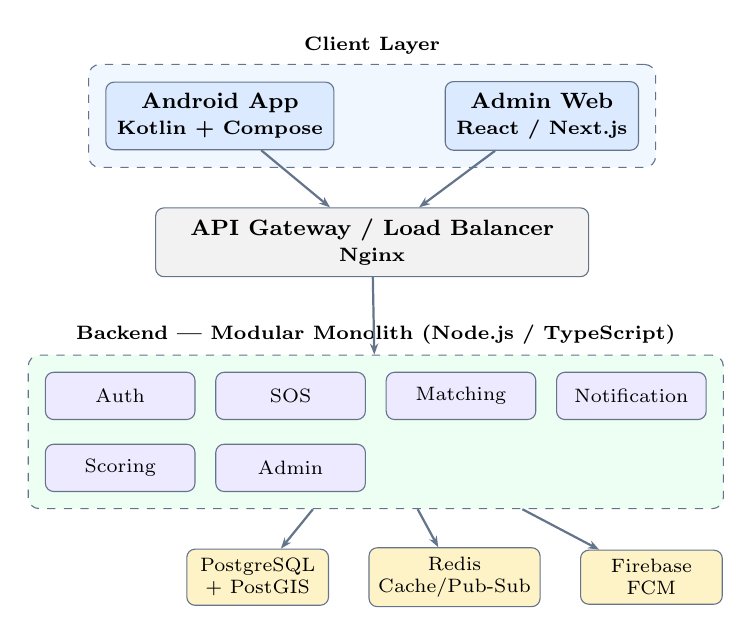
\begin{tikzpicture}[node distance=0.45cm and 0.3cm]
  \node[sysbox=clientbg] (android) {Android App\\{\scriptsize Kotlin + Compose}};
  \node[sysbox=clientbg, right=1.4cm of android] (admin) {Admin Web\\{\scriptsize React / Next.js}};
  \begin{scope}[on background layer]
    \node[fit=(android)(admin), fill=clientbg!40, draw=boxborder, dashed,
          rounded corners, inner sep=6pt,
          label={[font=\scriptsize\bfseries]above:Client Layer}] (clientlayer) {};
  \end{scope}

  \node[sysbox=white!90!gray, below=0.5cm of clientlayer, minimum width=5.5cm]
    (gw) {API Gateway / Load Balancer\\{\scriptsize Nginx}};
  \node[modbox, below=1.2cm of gw, xshift=-3.2cm] (auth)  {Auth};
  \node[modbox, right=0.25cm of auth]              (sos)   {SOS};
  \node[modbox, right=0.25cm of sos]               (match) {Matching};
  \node[modbox, right=0.25cm of match]             (notif) {Notification};
  \node[modbox, below=0.3cm of auth]               (score) {Scoring};
  \node[modbox, right=0.25cm of score]             (adm)   {Admin};
  \begin{scope}[on background layer]
    \node[fit=(auth)(sos)(match)(notif)(score)(adm),
          fill=backbg!50, draw=boxborder, dashed, rounded corners, inner sep=6pt,
          label={[font=\scriptsize\bfseries]above:Backend --- Modular Monolith (Node.js / TypeScript)}]
          (backend) {};
  \end{scope}

  \node[dbbox, below=0.5cm of backend, xshift=-1.5cm] (pg)
    {PostgreSQL\\+~PostGIS};
  \node[dbbox, right=0.5cm of pg]    (redis) {Redis\\Cache/Pub-Sub};
  \node[dbbox, right=0.5cm of redis] (fcm)   {Firebase\\FCM};

  \draw[arrowstyle] (android) -- (gw);
  \draw[arrowstyle] (admin)   -- (gw);
  \draw[arrowstyle] (gw)      -- (backend);
  \draw[arrowstyle] (backend) -- (pg);
  \draw[arrowstyle] (backend) -- (redis);
  \draw[arrowstyle] (backend) -- (fcm);
\end{tikzpicture}
\caption{ResQNet High-Level System Architecture}
\label{fig:arch}
\end{figure}

% ── 2. Motivation ───────────────────────────────────────────────
\section{Motivation}
Emergency response in many communities suffers from delayed reaction times, lack of inter-agency coordination, and over-dependence on formal services (ambulances, fire brigades) that may not reach the scene within the critical first few minutes. Studies show that bystander intervention during the first 4--6 minutes of a cardiac arrest can double or triple survival rates~[1]. Yet this pool of potential first responders --- neighbours with first-aid training, bystanders near an accident, off-duty paramedics --- remains largely untapped because no coordinated, location-aware dispatch platform exists for them. ResQNet is motivated by three converging trends:
\begin{enumerate}[nosep, leftmargin=1.4em]
  \item \textbf{The ``golden window'' imperative} --- Professional response times average 7--14 minutes in urban areas and far longer in rural settings; a volunteer already on-scene can bridge this gap.
  \item \textbf{Ubiquitous smartphones} --- Over 80\% of the Indian population now carries a GPS-enabled device, making real-time geolocation and push notifications technically feasible at scale.
  \item \textbf{Community resilience models} --- Platforms such as PulsePoint~[1] and Ushahidi~[4] have demonstrated that crowdsourced crisis response is both viable and effective.
\end{enumerate}

% ── 3. Literature Review ────────────────────────────────────────
\section{Literature Review}
\textbf{Volunteer dispatch systems.}
PulsePoint~[1] alerts CPR-trained citizens when a cardiac arrest occurs nearby, and controlled studies report statistically significant reductions in bystander-to-patient time. GoodSAM extends this concept to broader medical emergencies using video triage~[7].

\textbf{Crowdsourced crisis platforms.}
Howe~[2] formalised the ``crowdsourcing'' paradigm, which Ushahidi~[4] operationalised for disaster mapping during the 2010 Haiti earthquake, validating community-sourced geospatial reporting at scale. Meier~[4] further documents how digital volunteer networks coordinate relief logistics.

\textbf{Trust and reliability.}
Tatem et al.~[3] highlight how geographic mobility patterns affect volunteer availability and trustworthiness. More recent work on reputation scoring in sharing-economy platforms (e.g., Uber, Airbnb) provides design patterns for computing dynamic reliability scores based on response history, completion rates, and peer feedback~[8].

\textbf{Technology enablers.}
PostGIS~[6] provides sub-millisecond spatial queries (\texttt{ST\_DWithin}, \texttt{ST\_Distance}) essential for proximity matching at scale. Firebase Cloud Messaging~[5] offers a cross-platform push channel with delivery confirmation. Redis Pub/Sub enables low-latency event streaming between backend modules.

\textbf{Identified gap.}
Existing platforms are either event-specific (cardiac only), region-locked, or focused on post-disaster mapping rather than real-time volunteer dispatch. No unified, open-source system combines (a) geospatial volunteer matching, (b) reliability scoring, (c) live SOS lifecycle tracking, and (d) an administrative oversight dashboard --- the niche ResQNet targets.

% ── 4. Problem Definition ───────────────────────────────────────
\section{Problem Definition}
When emergencies occur, formal response systems are often delayed due to high call volume, traffic congestion, or geographic remoteness. There is no widely adopted platform that enables community volunteers to (i)~receive proximity-based emergency alerts, (ii)~accept or decline a request, and (iii)~coordinate with the requester in real time. Furthermore, the trustworthiness and competence of volunteer responders must be quantified to prevent misuse and prioritise reliable individuals.

ResQNet addresses this problem by designing a real-time volunteer dispatch system that:
\begin{enumerate}[nosep, label=(\alph*), leftmargin=1.6em]
  \item \textbf{Locates and ranks} nearby available volunteers using PostGIS \texttt{ST\_DWithin} geospatial indexing.
  \item \textbf{Notifies instantly} via Firebase Cloud Messaging push notifications.
  \item \textbf{Tracks the full lifecycle} of each SOS --- from trigger through volunteer acceptance, en-route tracking, and resolution.
  \item \textbf{Maintains a reliability score} per volunteer, computed from response rate, average response time, and post-incident feedback.
\end{enumerate}

% ── 5. Objectives ───────────────────────────────────────────────
\section{Objectives}
\begin{enumerate}[nosep, leftmargin=1.4em]
  \item Design and implement a \textbf{real-time SOS dispatch engine} using PostGIS \texttt{ST\_DWithin} to match requesters with the nearest available volunteers within seconds of an alert.
  \item Develop an \textbf{Android application} (Kotlin, Jetpack Compose) supporting dual requester/volunteer roles, featuring live location sharing, SOS status tracking, and FCM push notifications, following the Clean Architecture depicted in Figure~\ref{fig:android}.
  \item Build a \textbf{volunteer reliability scoring module} that ranks candidates on response rate, response latency, and post-incident ratings, ensuring accountability within the network.
  \item Deploy an \textbf{admin web dashboard} (Next.js) with live SOS monitoring, user management, analytics, and moderation capabilities.
  \item Architect the backend as a \textbf{modular monolith} (Node.js, TypeScript, PostgreSQL, Redis) designed for MVP delivery and structured for incremental horizontal scaling to 100\,K+ concurrent users.
\end{enumerate}

\vspace{0.1cm}
% ── Figure 2: Android Clean Architecture ─────────────────────────
\begin{figure}[h]
\centering
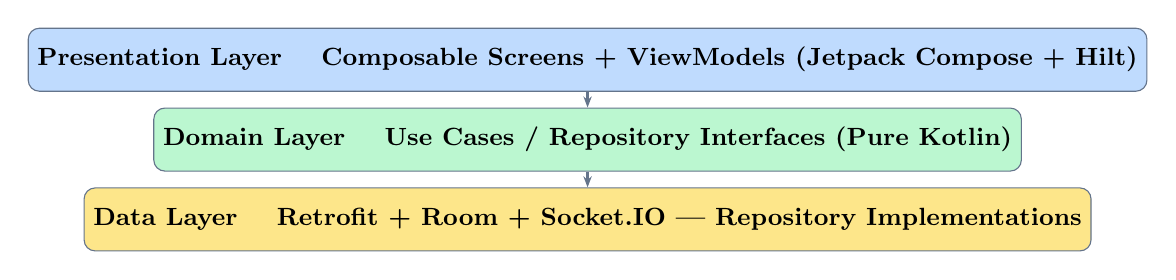
\begin{tikzpicture}
  \node[layerbox=layerA] (pres)
    {Presentation Layer \quad {\small Composable Screens + ViewModels (Jetpack Compose + Hilt)}};
  \node[layerbox=layerB, below=0.2cm of pres] (domain)
    {Domain Layer \quad {\small Use Cases / Repository Interfaces (Pure Kotlin)}};
  \node[layerbox=layerC, below=0.2cm of domain] (data)
    {Data Layer \quad {\small Retrofit + Room + Socket.IO --- Repository Implementations}};
  \draw[arrowstyle] (pres.south)   -- (domain.north);
  \draw[arrowstyle] (domain.south) -- (data.north);
\end{tikzpicture}
\caption{Android App --- Clean Architecture Layers}
\label{fig:android}
\end{figure}

% ── 6. Proposed Methodology ─────────────────────────────────────
\section{Proposed Methodology}
The development follows an iterative, sprint-based methodology with four major phases:

\textbf{Phase 1 --- Requirements \& Design.}
System requirements were gathered through a survey of existing emergency-response literature and informal interviews with first-aid volunteers. The system architecture (Figure~\ref{fig:arch}) was designed around a modular monolith to balance rapid prototyping with future decomposition into microservices.

\textbf{Phase 2 --- Backend \& Database.}
The API server is implemented in Node.js with TypeScript. PostgreSQL extended with PostGIS provides the persistence and geospatial query layer; a \texttt{geography} column on the \texttt{volunteers} table enables sub-millisecond radius searches via \texttt{ST\_DWithin}. Redis is used for session caching, rate-limiting, and Pub/Sub event distribution. Authentication uses JWT with refresh-token rotation.

\textbf{Phase 3 --- Mobile \& Web Clients.}
The Android application is built with Jetpack Compose following Clean Architecture (Figure~\ref{fig:android}): the \emph{Presentation} layer (Compose screens, ViewModels) depends only on the \emph{Domain} layer (use cases, repository interfaces), which is implemented by the \emph{Data} layer (Retrofit for REST, Room for offline cache, Socket.IO for real-time events). Dependency injection is handled via Hilt. The admin dashboard is a server-rendered Next.js application consuming the same REST API.

\textbf{Phase 4 --- Testing \& Deployment.}
Unit tests cover domain use cases; integration tests validate API endpoints with a dockerised test database. End-to-end SOS flows are verified on physical devices. Deployment targets a single VPS with Nginx reverse-proxy, with Docker Compose orchestrating the backend, PostgreSQL, and Redis containers.

% ── 7. Expected Outcomes ────────────────────────────────────────
\section{Expected Outcomes}
\begin{itemize}[nosep, leftmargin=1.4em]
  \item A fully functional Android application enabling users to trigger SOS alerts and nearby volunteers to accept and respond in real time.
  \item Average volunteer notification latency $<$ 3\,seconds from SOS trigger under normal network conditions.
  \item A reliability scoring algorithm that measurably prioritises volunteers with higher historical response rates.
  \item An admin dashboard providing real-time SOS monitoring, user analytics, and moderation tools.
  \item A documented, containerised deployment pipeline reproducible on commodity hardware.
\end{itemize}

% ── 8. References ───────────────────────────────────────────────
\section{References}
\begin{enumerate}[nosep, leftmargin=1.4em]
    \item[\lbrack 1\rbrack] T. D. Rea \textit{et al.}, ``CPR with Telephone Assistance from Emergency Medical Services Dispatchers,'' \textit{New England Journal of Medicine}, vol.~363, pp.~943--953, 2010.
    \item[\lbrack 2\rbrack] J. Howe, ``The Rise of Crowdsourcing,'' \textit{Wired Magazine}, vol.~14, no.~6, pp.~1--4, 2006.
    \item[\lbrack 3\rbrack] A. Tatem, S. Hay, and D. Rogers, ``Global traffic and disease vector dispersal,'' \textit{Proc. Natl. Acad. Sci.}, vol.~103, no.~16, pp.~6242--6247, 2006.
    \item[\lbrack 4\rbrack] P. Meier, \textit{Digital Humanitarians: How Big Data Is Changing the Face of Humanitarian Response}. CRC Press, 2015.
    \item[\lbrack 5\rbrack] Google LLC, ``Firebase Cloud Messaging,'' \textit{Firebase Documentation}, 2024. [Online]. Available: \url{https://firebase.google.com/docs/cloud-messaging}
    \item[\lbrack 6\rbrack] PostGIS Development Team, ``PostGIS 3.x Reference Manual,'' 2024. [Online]. Available: \url{https://postgis.net/docs/}
    \item[\lbrack 7\rbrack] GoodSAM, ``GoodSAM Alerter --- Saving Lives with Technology,'' 2024. [Online]. Available: \url{https://www.goodsamapp.org}
    \item[\lbrack 8\rbrack] S. Tadelis, ``Reputation and Feedback Systems in Online Platform Markets,'' \textit{Annual Review of Economics}, vol.~8, pp.~321--340, 2016.
\end{enumerate}

\vspace{0.5cm}
\begin{tabular}{ p{5.5cm} p{5.5cm} p{5.5cm}}
\textbf{Kshitiz Raj} & \textbf{Sujal Agrawal}  & \textbf{Krishna Goswami}  \\
Signature 1 & Signature 2 &  Signature 3  \\ [30pt]
 & & \textbf{Mrs. Akansha Moral} \\
& & Signature \\  [30pt]
\end{tabular}
\end{document}
